\begin{figure*}[htb]
  \centering
  \begin{subfigure}[t]{0.33\textwidth}
    \centering
    \includegraphics[width=\textwidth]{figures/profile-mot.pdf}
    \caption{Pedestrian Detection}
    \label{fig:pd-profile}
  \end{subfigure}
  \hfill
  \begin{subfigure}[t]{0.33\textwidth}
    \centering
    \includegraphics[width=\textwidth]{figures/profile-darknet.pdf}
    \caption{Augmented Reality}
    \label{fig:ar-profile}
  \end{subfigure}
  \hfill
  \begin{subfigure}[t]{0.33\textwidth}
    \centering
    \includegraphics[width=\textwidth]{figures/profile-topk.pdf}
    \caption{Top-k}
    \label{fig:tk-profile}
  \end{subfigure}
  \caption{Application profiles.}
  \label{fig:all-profiles}
\end{figure*}

\newpage

\section{Evaluation}
\label{sec:evaluation}

In this section, we show our evaluations of \sysname{}. The results are
summarized as follows.

\begin{itemize}
\item[\autoref{sec:application-profiles}] \sysname{} generates Pareto-optimal
  profiles with precision and fine granularity (\autoref{fig:all-profiles}).
\item[\autoref{sec:online-profiling}] Our parallel and partial profiling enables
  fast online profiling with about 10\% GPU time (\autoref{fig:parallel},
  \autoref{fig:online-tricks}).
\item[\autoref{sec:runtime-adaptation}] At runtime, \sysname{} applications
  achieve sub-second latency and little accuracy drop
  (\autoref{fig:all-runtime}).
\item[\autoref{sec:multi-task-alloc}] \sysname{} profiles allow equal-accuracy
  bandwidth allocation among multiple streams (\autoref{fig:multitask}).
\end{itemize}

\subsection{Application Profiles}
\label{sec:application-profiles}

Our system learned the application profiles for all three applications (shown in
\autoref{fig:all-profiles}). From these profiles, we make the following three
observations:

\para{Little accuracy drop across three or four orders of magnitude}. This
allows operating in an acceptable state even under bandwidth scarcity.

\para{Optimal strategy is achieved with multiple dimensions.} In each profile,
in addition to the Pareto-optimal strategies, we show the performance if only
one dimension is tuned. As show in the figure, they almost always lead to a
sub-optimal performance.

\para{The effect of each dimension is different}. Different dimensions have
different impact for the same application. For pedestrian detection, tuning
resolution leads to a quicker degradation in comparison to tuning frame
rate. The same dimension has different impact for different applications. If we
compare two video analytics applications, pedestrian detection and augmented
reality, we see how tuning each dimension affects the performance differently.

\lipsum[1-2]

\subsection{Efficient Online Profiling}
\label{sec:online-profiling}

This section focuses on the AR application as a case study. First, we validate
the necessity for online profiling. We compare two adaptation scheme: one with
the offline learned profile; the other enabled with online
profiling. \autoref{fig:online-tricks} offline and online. Initially, both
schemes work similarly. Overtime, when the data distribution changes, the
offline-learned profile doesn't match with the newly generated data, leading to
accuracy deterioration. System enabled with online profiling is able to track
the data and offers high accuracy.

\autoref{fig:parallel} shows how much profiling is needed with more machines and
use different schedulers. First, we see that the parallel execution reduces the
execution time. Besides, our profiling scheduling improves the profiling
efficiency with 2x time reduction in comparison to baseline schedulers.

\autoref{fig:online-tricks} illustrates how the application behaves with
different model. With partial profiling, such as every five seconds worth of
data out of 30 seconds; there is a delay in reacting to model change. With
triggering, the profile closesly resembles the always online case.

\begin{figure}
  \centering
  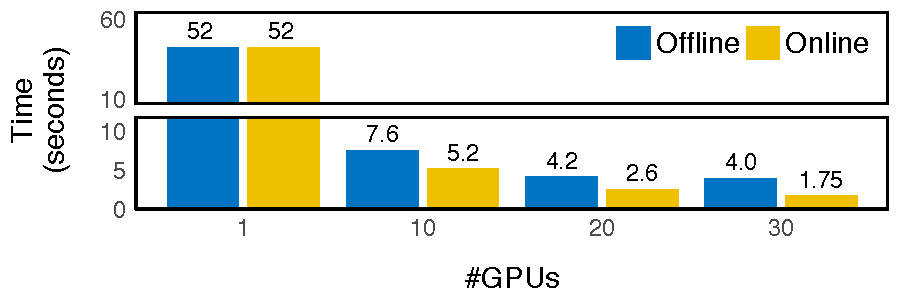
\includegraphics[width=0.8\columnwidth]{figures/parallel.pdf}
  \caption{Degradation-aware parallel scheduling}
  \label{fig:parallel}
\end{figure}

%% Offline: 0
%% Online: 1 frame (1852.21 GPU * seconds)
%% Online (1/10)   (185.2 GPU * seconds)
%% Trigger         ( GPU * seconds)

\lipsum[1-2]

\begin{figure}
  \centering
  \includegraphics[width=\columnwidth]{figures/online-profiling.pdf}
  \caption{Trigger-based profiling}
  \label{fig:online-tricks}
\end{figure}

\begin{table}[t]
  \centering
  \begin{tabular}{c|c|c|c}
    \hline
    offline & online & online (partial) & online (trigger) \\
    \hline
    0       & 1852 (ms)   & 617 (ms)              & 223 (ms) \\
    \hline
  \end{tabular}
  \caption{Online Profiling Time}
  \label{tab:online}
\end{table}

\begin{figure*}[!htb]
  \begin{subfigure}[t]{0.3\textwidth}
    \centering
    \includegraphics[width=\textwidth]{figures/runtime-mot-verticle.pdf}
    \caption{Pedestrian Detection}
    \label{fig:pd-runtime}
  \end{subfigure}
  \hfill
  \begin{subfigure}[t]{0.3\textwidth}
    \centering
    \includegraphics[width=\textwidth]{figures/runtime-darknet-verticle.pdf}
    \caption{Augmented Reality}
    \label{fig:ar-runtime}
  \end{subfigure}
  \hfill
  \begin{subfigure}[t]{0.3\textwidth}
    \includegraphics[width=\textwidth]{figures/runtime-topk-verticle.pdf}
    \caption{Top-k}
    \label{fig:tk-runtime}
  \end{subfigure}
  \caption{Application profiles.}
  \label{fig:all-runtime}
\end{figure*}

\subsection{Runtime Adaptation}
\label{sec:runtime-adaptation}

To evaluate the runtime behavior, we conduct controlled experiments using four
geo-distributed worker nodes from Amazon EC2 (t2.large instances) and an
aggregation server from our institute. For each experiment, worker nodes
transmit test data for about 10 mins. During each session, we use Linux
\texttt{tc} utility to adjust outgoing bandwidth to experiment with network
resource variation.

We show three aspects of the system: throughput, latency and application
accuracy. We compare our system with baseline systems that directly uses TCP and
UDP. In all three applications, the raw data streams are orders of magnitude
larger. While our system can adapt the rate, it could be unfair to baseline
solutions. We adjust the default degradation operation so that TCP and UDP would
work just fine when in normal cases; in this way, we make fair comparison. In
the case of UDP, shaping at the source doesn't emulate the packet loss behavior
with out-of-order delivery. We use \texttt{netem} to control packet loss rate to
match the desired shaping bandwidth.

From the throughput figure, we see how traffic shaping start, more severe
traffic shaping and traffic shaping stop affect the throughput. Notice that
after the traffic shaping stops, TCP has a ``catch-up'' phase where it's sending
all the queued items as fast as possible. Because of the queuing, TCP suffers
from an increased latency (as seen in the latency figure). But the data is
maintained at high fidelity in TCP, so the accuracy is always high. For UDP,
there is no explicit latency increase, but the accuracy drop is drastic during
traffic shaping.

Our run time adaptation achieves the balance between these two extremes: it has
low-latency (under 1 seconds) and high accuracy (above 85\%).

\lipsum[1-2]

\newpage

\subsection{Multi-task Allocation}
\label{sec:multi-task-alloc}

At last the profile is useful for scheduling multiple stream processing
analytic. Applications doesn't behave well if they don't have the
adaptation. When their adaptation is turned on, but multiple tasks are
competing, some will suffer from the fair adaptation. This motivates us to
explore the multi-task scheduling.

There are mainly two schemes we are considering: (1) maximize the
\textit{minimum} utility (for \textit{MaxMin} fairness); (2) maximize the total
utility (for \textit{MaxTotal} performance). \autoref{fig:multitask} shows the
total utility of the baseline scheme and our two scheduling schemes.

\begin{figure}
  \centering
  \begin{subfigure}[t]{0.49\columnwidth}
    \centering
    \includegraphics[width=\textwidth]{figures/multitask-eq-bw.pdf}
    \caption{Equal Bandwidth}
    \label{fig:eq-bw}
  \end{subfigure}
  \hfill
  \begin{subfigure}[t]{0.49\columnwidth}
    \centering
    \includegraphics[width=\textwidth]{figures/multitask-eq-acc.pdf}
    \caption{Equal Acc}
    \label{fig:eq-acc}
  \end{subfigure}
  \caption{Multitask Allocation.}
  \label{fig:multitask}
\end{figure}

\newpage

%%% Local Variables:
%%% mode: latex
%%% TeX-master: "sosp17"
%%% End:
